\documentclass[UTF8,a4paper]{ctexart}
\usepackage[margin=1in]{geometry}
\usepackage{graphicx,float,array,color,bm,amsmath,amssymb,hyperref}
\pdfstringdefDisableCommands{\let\bm\@firstofone}
\hypersetup{hidelinks}
\author{qhy}
\date{\today}
\title{Multiple Kernel Learning}
\begin{document}
    \maketitle
    \tableofcontents
    \newpage
    \section{Multiple Kernel Learning}
        \subsection{核方法原理}
        给定样本$\mathcal{D} = \{(\bm{x_1} , y_1),\cdots,(\bm{x_n} , y_n)\}$,求从输入$\bm x$ 到$y$的映射。

        可以先进行一次非线性映射$\Phi:\bm x\to\phi(\bm x)$,把$\bm x$映射到高维空间

        然后再在数据新的表示方法$\mathcal{D'} = \{(\bm{\phi(x_1)} , y_1),\cdots,(\bm{\phi(x_n)} , y_n)\}$上考虑原来的机器学习问题。

        和函数把非映射和特征空间中的两个向量的内积两步集合起来,使得非线性映射隐式地进行。
        具体地说,使用核函数来进行高维空间的内积计算,通过对低维空间上的运算来计算高维空间的内积,
        而不是直接使用高维空间的表示进行内积,避免了维数灾难\footnote{在高维情形下出现的数据样本稀疏,距离计算困难等问题,是所有机器学习方法共同面临的严重障碍,被称为"维数灾难"(curse of dimensionality)}。

        \subsection{Mercer条件}
        \textbf{Mercer条件:}设$X$是$R^n$的一个紧子集,$k:X\times X \to R$是一个连续的对称函数,
        如果它在希尔伯特空间上的积分算子满足积分正定条件:
        \begin{equation}
            \forall f \in L_2(X) , \int_{X\times X} k(\bm x , \bm z)f(\bm x)f(\bm z)d\bm x d\bm z
        \end{equation}
        那么一定存在一个特征空间$F$和一个映射$\Phi:X\to F$,使得
        \begin{equation}
            k(\bm x, \bm z) = \Phi(\bm x)\times \Phi(\bm z)
        \end{equation}

        \subsection{核函数的性质}
        \begin{itemize}
            \item 容许核\footnote{满足Mercer条件的和函数称为容许核}的正系数线性组合是容许核。
            \item 容许核的乘积是容许核。
            \item 函数乘积的积分是容许核。
        \end{itemize}

        \subsection{多核学习}
            多核学习:使用多个核的线性或非线性组合来构造新的核,然后使用新的核考虑原来的问题。

            以简单地线性组合为例:

            新的核函数为:
            \begin{equation}
                \bm K' = \sum_{i = 1}^n \beta_i\bm K_i
            \end{equation}
            那么对于样本$\bm X$和标签$\bm Y$来说,最小化的问题可以写成以下形式:
            \begin{equation}
                \min_{\beta , c} E(Y,K'c) + R(K,c)
            \end{equation}
            其中,$\bm E$是误差函数,$\bm R$是正则项。

            \subsubsection{组合方式}
                多核学习,简单地看,就是多个核的线性和非线性组合(合成出一个新的核),因此,组合的方式是一个重要因素。根据核函数的性质,我们有加和和乘积两个基本方式。

                举个例子:
                \begin{itemize}
                    \item \textbf{pairwise kernels}
                    \begin{equation}
                        k((x_{1i},x_{1_j}) , (x_{2i},x_{2j})) = k(x_{1i} , x_{2i})k(x_{1j} , x_{2j}) + k(x_{1i,x_{2j}})k(x_{1j},x_{2i})
                    \end{equation}
                    \item \textbf{线性组合}
                    \begin{figure}[H]
                        \centering
                        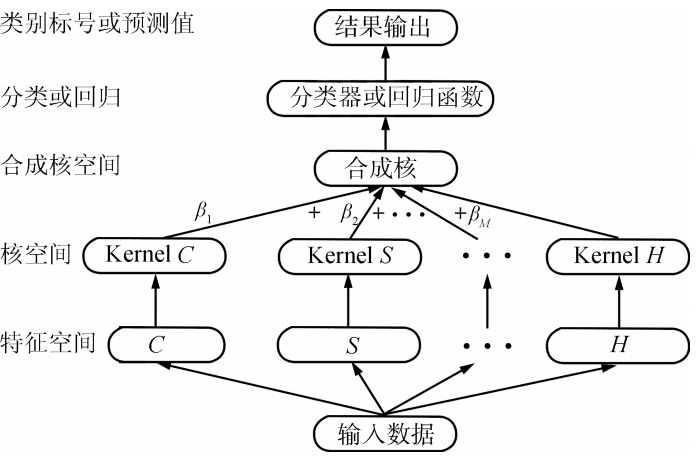
\includegraphics[scale = 0.3]{assets/MultipleKernelLearning_96672.png}
                        \caption{多核函数线性组合合成示意图}
                    \end{figure}
                \end{itemize}
            \subsubsection{启发式规则}
                启发式规则:简单地说,就是给多核增加各种参数,使用学习或者启发式的方法来定义各种参数。

                \textbf{例1:}

                假设:\begin{itemize}
                    \item $\bm \pi_m$表示只使用第$m$个核函数的情况下的精度
                    \item $\delta$表示某个阈值
                \end{itemize}
                定义:
                \begin{equation}
                    \beta_m = \frac{\bm \pi_m - \delta}{\sum_{h = 1}^n(\bm \pi_h - \delta)}
                \end{equation}

                \textbf{例2}

                定义相似度:
                \begin{equation}
                    A(\bm K_1 , \bm K_2) = \frac{<\bm K_1 , \bm K_2>}{\sqrt{<\bm K_1 , \bm K_1><\bm K_2 , \bm K_2>}}
                \end{equation}
                则:
                \begin{equation}
                    \beta_m = \frac{A(\bm K_m , \bm Y \bm Y^T)}{\sum_{h = 1}^n A(\bm K_h , \bm Y\bm Y^T)}
                \end{equation}

                {\color{red}为什么是$\bm Y\bm Y^t$}

            \subsubsection{贝叶斯方法}
            贝叶斯方法:给需要学习的参数一个先验分布

            举个例子:

            最终预测函数为:
            \begin{equation}
                f(\bm x) = \sum_{i = 0}^n \alpha_i \sum_{m = 1}^p \eta^m \bm K_m(\bm x_i^m , \bm x^m)
            \end{equation}
            假设,$\bm \eta$为狄利克雷分布,$\bm \alpha$为高斯分布

            \subsubsection{Boosting 方法??????}

        \subsection{多尺度核方法}
        多尺度核方法,使用尺度大的基核函数对平缓变换的样本进行分类,使用尺度小的基和核函数对剧烈变化的样本进行分类。

            \subsubsection{具有多尺度表示能力的核函数}
            多尺度核方法的基础就是要找一组能具有多尺度表示能力的核函数,在被广泛使用的核函数中,RBF核
            \begin{equation}
                k(\bm x ,\bm z) = exp(\frac{\|\bm x - \bm z\|^2}{2\sigma^2})
            \end{equation}
            是最受欢迎的。

            以此核为例,$\sigma$取不同的值表示不同的尺度。$\sigma$较大的时,用来对那些平缓变化的样本进行分类,小的时候对剧烈变换的样本进行分类。

            {\color{blue}k从一定程度上也是描述样本之间的相似度,当$\sigma$大的时候,表示相似,因此可以对平缓变化的样本进行分类。}

            \subsubsection{多尺度核的学习方法}

            考虑两个尺度的核$k_1$和$k_2$的分类问题,我们要合成的决策函数为以下形式:
            \begin{equation}
                f(\bm x) = f_1(\bm x) + f_2(\bm x)
            \end{equation}
            其中,
            \begin{equation}
                f_1(\bm x) = \sum_{i = 1}^N \alpha_ik_1(\bm x_i , \bm x) + b_1
            \end{equation}
            \begin{equation}
                f_2(\bm x) = \sum_{i = 1}^N \beta_ik_2(\bm x_i , \bm x) + b_1
            \end{equation}

            {\color{blue}这里一个尺度的核函数表示一个输出值,最终是值的叠加,而不是前面的核的叠加}

            这里假设$k_1$是大尺度的核,$k_2$是小尺度的核。

            首先通过大尺度的单核$k_1$来构造$f_1(\bm x)$来拟合光滑的区域,再在$f_1{\bm x}$的基础上,使用尺度较小的核$k_2$构造$f_2{\bm x}$,这样$f_1(\bm x) + f_2{\bm x}$比$f_1{\bm x}$具有更好的拟合性能。

\end{document}
